%%%%%%%%%%%%%%%%%%%%%%%%%%%%%%%%%%%%%%%%%%%%%%%%%%%%%%%%%%%%%%%%%%%
%
% This is a general template file for the LaTeX package SVJour3
% for Springer journals.          Springer Heidelberg 2010/09/16
%
% Copy it to a new file with a new name and use it as the basis
% for your article. Delete % signs as needed.
%
% This template includes a few options for different layouts and
% content for various journals. Please consult a previous issue of
% your journal as needed.
%
%%%%%%%%%%%%%%%%%%%%%%%%%%%%%%%%%%%%%%%%%%%%%%%%%%%%%%%%%%%%%%%%%%%
%
\RequirePackage{fix-cm}
%
\documentclass[twocolumn]{svjour3}
%
\smartqed
%
\usepackage{graphicx}
\usepackage[T1]{fontenc}
\usepackage{hyperref}
\usepackage[round, sort&compress, numbers]{natbib}
\usepackage{multirow}
\usepackage{graphicx}
\usepackage{units}
\usepackage{color}
\usepackage{colortbl}
\usepackage{xspace}
\usepackage{epsfig}
%
\DeclareRobustCommand\IPCClongname{}
\setcounter{secnumdepth}{5}
%
% please place your own definitions here and don't use \def but \newcommand{}{}
\newcommand{\pmlib}{\texttt{pmlib}\xspace}
\newcommand{\monch}{\textsc{Monch}\xspace}
\newcommand{\pilat}{\textsc{Pilatus}\xspace}
\newcommand{\tinto}{\textsc{Tintorrum}\xspace}
\newcommand{\cosmoart}{\textsc{Cosmo-Art}\xspace}
%
% Insert the name of "your journal" with
% \journalname{myjournal}
%
\begin{document}

\title{Evaluating the Performance and Energy Efficiency of the
  \textsc{COSMO-ART} model system}
%\thanks{}
%\subtitle{}

%\titlerunning{Short form of title} % if too long for running head

\author{Joseph~Charles \and William~Sawyer \and Manuel~F.~Dolz \and
  Sandra~Catal\'an}

%\authorrunning{Short form of author list} % if too long for running
%head

\institute{J.~Charles, W.~Sawyer
	\at Swiss National Supercomputing Centre (CSCS)
	\\ CH-6900 Lugano, Switzerland
 	\\ E-mails:~{\{joseph.charles,william.sawyer\}@cscs.ch}
        \and M.~F.~Dolz
        \at Dept. of Informatics, University of Hamburg (UHAM)
	\\ DE-22527 Hamburg, Germany
        \\ \email{manuel.dolz@informatik.uni-hamburg.de}
        \and S.~Catal\'an
        \at Jaume I University of Castell\'on (UJI)
	\\ ES-12071 Castell\'on, Spain
        \\ \email{catalans@icc.uji.es}
}

\date{Received: date / Accepted: date} % The correct dates will be
                                       % entered by the editor

\maketitle

\begin{abstract}
  In this  paper we investigate  the energy footprint  and performance
  profiling  of  \textsc{COSMO-ART} on  various  HPC platforms.   This
  model is an  extension of the operational weather  forecast model of
  the German  weather service (DWD),  developed for the  evaluation of
  the interactions  of reactive gases  and aerosol particles  with the
  state of  atmosphere at  the regional scale.   Different measurement
  devices and  energy-aware techniques are described  to evaluate both
  time and  energy to  solution of the  considered application  and to
  gain detailed insights into power and performance requirements.  Our
  motivation  is to  improve  corresponding code  sections to  sustain
  performance  while minimising energy-to-solution.   This preliminary
  work  sets the  basis for  subsequent studies  to  tackle challenges
  related  to  energy  efficient  high performance  computing  in  the
  framework of the Exa2Green project \citep{EXA2GREEN}.

\keywords{High performance computing  \and Energy-aware computing \and
  Green computing  \and Numerical weather  prediction \and Atmospheric
  chemistry  \and  Aerosols  modelling  \and  Profiling  methods  \and
  Benchmark  analysis  \and   \textsc{COSMO-ART}  coupled  model  \and
  Time-to-solution \and Energy-to-solution \and Xeon processor}
% \PACS{PACS code1 \and PACS code2 \and more} 
% \subclass{MSC code1 \and MSC code2 \and more}
\end{abstract}

\section{Introduction}
\label{intro}
While anthropogenic greenhouse gas emissions are driving unprecedented
major  climate  changes  since   the  mid-20$^{th}$  Century,  one  factor
overwhelmingly  affects  the  uncertainty  in  determining  human-induced
radiative  forcing:  the  effects   of  aerosols  in  the  atmosphere.
Although they  are not considered  heat-trapping greenhouse  gases and
have  shorter  atmospheric lifetimes,  aerosols  significantly modify  the
global   radiation   budget   \citep{IPCC-2013}.   Enhanced   aerosols
concentrations impact the climate  system by scattering and absorption
of solar radiation, thereby exerting a direct radiative forcing; or by
modifying cloud  properties,  cloud  fraction and  surface
albedo,  causing  a  negative  indirect  radiative  forcing.   Despite
considerable  progress in  global aerosol  modelling \citep{Mann-2013}
and  measurement-based  assessments,  large  uncertainties  remain  in
current  estimates  of  aerosol radiative  forcing  \citep{Myhre-2013,
IPCC-2013,  Lee-2013,   Randles-2013,  Rosenfeld-2013,  Sherwood-2013,
Stier-2013}.

Hence to  improve our understanding of  aerosol-cloud interactions and
reduce  these  uncertainties,  the  research  community  is  making  a
concerted international  effort to represent  the underlying physical,
chemical  and aerosol dynamical  processes through  numerical chemical
transport  models (CTMs)  such  as ART  (Aerosols  and Reactive  Trace
gases),   developed   at  the   Karlsruhe   Institute  of   Technology
(KIT)  \citep{Vogel-2009,  Bangert-2011,  Knote-2013}.  This  regional
scale modelling system is coupled  with the operational  weather forecast
model  \textsc{Cosmo}  \citep{Baldauf-2011},  jointly developed and used by  a
consortium of European weather centers, as well as utilised in a climate version
by the wider research community.

The extended  atmospheric model \textsc{Cosmo-art}  is com\-put\-ationally
much  more  demanding than  \textsc{Cosmo}  since  a  large number  of
additional  tracers and  processes have  to be  considered.   Thus the
model  is currently  severely limited  in terms  of applicability  and
expensive in terms of energy consumption.  Although \textsc{Cosmo} has
recently been ported to GPUs \citep{Gysi-2014, Lapillonne-2014} within
the framework of the  High Performance and High Productivity Computing
(HP2C) Initiative  \citep{HP2C} to optimise it  for computational and
energy efficiency,  significant investments in ART  are still required
to take it  to a similar level.  The  efficiency of \textsc{Cosmo-art}
is being  addressed in the  EU Exa2Green project  \citep{EXA2GREEN} to
deliver a  prototype code, which  provides an energy efficiency  of at
least five times the  baseline value.  Such an implementation would
allow  the  community  to  investigate critical  questions  at  higher
resolution  and   over  longer  periods,   at  reduced  cost   to  the
environment.

This  work is  organized as  follows: in  Sec.~\ref{sec:1} we  give an
overview  of  related  work,   then  in  Sec.~\ref{sec:2}  we  briefly
introduce \textsc{Cosmo-art}  and specify its  technical setup related
to  the investigated  performance and  energy evaluation  methods.  In
Sec.~\ref{sec:3}   we  describe   HPC  platforms,   power  measurement
equipments   and  software  environment   employed  to   conduct  this
benchmarking study.  Sec.~\ref{sec:4}  presents performance and energy
requirements  of the  baseline on  these architectures  and highlights
areas where improvements will be necessary for the subsequent baseline
refactoring.   Finally,  we  conclude in Sec.~\ref{concl} with some 
implications for the Exa2Green project and give an outlook for future
research.


\section{Related work}
\label{sec:1}
While the  TOP500 list was  introduced over 20  years ago to  rank the
performance of HPC systems worldwide, it is quite recently that energy
efficiency  become  a  critical  constraint  in the  way  to  exascale
computing.   Since 2007,  the Green500  power  measurement methodology
encourages the design,  procurement and management of energy-efficient
infrastructures   to  contain   performance  in   an   affordable  and
competitive  power envelope.   However, the  state-of-the-art research
assessing performance  and energy efficiency of  applications is still
scarce.

\emph{Padoin et al.}   \cite{Padoin-2013} investigate performance and
power  consumption  of  an  agroforestry  application  and  show  that
changing workload  can drastically improve energy efficiency  of CPU +
GPU heterogeneous architectures.

\emph{Ou  Pang et  al.}   \cite{Ou-2012} compare  ARM  and Intel  x86
workstations  clusters  and   conclude  that  ARM-based  clusters  are
advantageous  with   lightweight  applications  in   terms  of  energy
efficiency.

\emph{G\"oddeke et al.}  \cite{Goddeke-2013} evaluate weak and strong
scalability of PDE solvers on a cluster of 96 ARM dual-core processors
and demonstrate  that the ARM-based  cluster can be more  efficient in
terms of energy-to-solution compared to x86-based cluster.

\emph{Wittmann  et  al.}   \cite{Wittmann-2013}  perform  a  thorough
analysis of  a lattice-Boltzmann method based CFD  simulation on Intel
Sandy   Bridge  processors   and  show   extrapolated  results   on  a
petascale-class machine.

% \emph{Cumming  et  al.}  \cite{Cumming-2014}  present  a simple  and
% practical  methodology  looking at  energy  minimization  that can  be
% applied to various applications.


\section{The \textsc{COSMO-ART} model system}
\label{sec:2}
\subsection{Model Description}
\label{subsec:1.1}

The model  system \cosmoart described  in \cite{Vogel-2009},
is  a  regional to  continental  scale  model  coupled online  to  the
\textsc{Cosmo}   numerical  weather   prediction  and   climate  model
\cite{Baldauf-2011}.   It   incorporates  sophisticated  modules  for
gaseous  chemistry   and  aerosol  dynamics  and   allows  the  online
calculation of  reactive trace  substances and their  interaction with
the  atmosphere.    Detailed  model   description  can  be   found  in
\cite{Bangert-2012, Knote-2011, Knote-2013}.

\subsection{Model Setup}
\label{subsec:1.2}

Establishing effective energy performance benchmarking of a code under
intense development  such as \cosmoart is  a challenging task
because of  the absolute necessity  that results must  be reproducible
within  an  expected  variance  for  the  duration  of  the  Exa2Green
pro\-je\-ct.  To   define  a  baseline,   it  was  necessary  to   find  a
run-configuration  capable  of   being  recreated  in  all  subsequent
versions.  Here  we give a brief  overview of the model  setup for our
performance and energy efficiency evaluation.

Three-dimensional simulations are performed over large parts of Europe
and the Mediterranean~Sea for April 13$^{th}$ 2010, near the equinox, in order to approximately
have a half  day  of  sun  exposure and  therefore  ensure  a typical
activation of the chemistry cycle.  The calculation domain corresponds
to the CORDEX-EU-44 domain and is covered by a grid of $222\times 216$
points with  a horizontal resolution of  $0.22\,^{\circ}$, i.e., 50~km
in  both directions  and 40~vertical  layers.  These  24-hour forecast
simulations  are not  preceded  by  a spin-up  phase  to build up  the
simulated gaseous and  aerosol concentrations.  This condition means 
that the model initialization needs a period of adjustment to reach its equilibrium  state and minimize  the effect of
initial conditions for gases and aerosols on the model predictions.

The meteorological initial and boundary conditions are obtained by the
the ECMWF  global spectral model IFS  with an update  frequency of 3h.
Boundary data  for gas-phase species are taken  from IFS-MOZART output
at  6h temporal resolution.   The model  setup incorporates  34~2D and
45~3D  fields to  be written  out  every hour  and is  devoid of  data
assimilation methods.

The considered  \cosmoart model  system is configured  with a
semi-Lagrangian    horizontal   advection    sche\-me    with   tricubic
interpolation  and selective filling  diffusion option  in combination
with   the   dynamical    core   using   Runge-Kutta   time   stepping
\cite{COSMO-PartI-2011}.    It  also   makes  use   of   the  Kinetic
PreProcessor solver (KPP) for  the solution of atmospheric chemistry
ordinary  differential equations \cite{Damian-2002}.   Concerning the
modelling  of  wet  deposition  in  aerosols, the  baseline  has  only
indirect  cloud feedbacks  but  does not  include in-cloud  scavenging
(rainout) and below-cloud  scavenging (washout) yet.  Amongst physical
parameterizations,   precipitation  formation   is   performed  by   a
two-moment cloud microphysics.


\section{Environment setup}
\label{sec:3}
\subsection{Hardware platforms}
\label{subsec:3.1}

Benchmarks presented  in this work  were performed on  three different
platforms  and can  be reproduced  within an  expected  variance, thus
allowing a  fair comparison between the baseline  and future milestone
versions of \cosmoart:

\begin{itemize}
\item \monch is  a 10-rack NEC-provided clus\-ter at  CSCS composed by
  384   nodes  grouped  in  312  standard  compute  nodes,  24
  large-memory compute nodes,  24 huge-memory nodes, 16 administration
  nodes and 8 servers to provide I/O to Lustre.
  % and  utilized  by  members  of  the  Swiss  Platform  for  Advanced
  % Scientific Computing (PASC) project~\cite{PASC}.  
Each standard  compute node  is comprised of  two Intel Xeon Ivy Bridge EP
E5-2660v2  ten-core processors  operating at  2.2\,GHz,  equipped with
32\,GB  of DDR3 1600\,MHz  RAM and  connected via  InfiniBand Mellanox
SX6036 and FDR switches.  For our experiments, only a subset of 52 was used. %
% only a full rack constituted exclusively of 52 nodes was used.
  % \monch is  slated to stay  in service without hardware  upgrade for
  % the  duration  of  the  Exa2Green project,  allowing  an  identical
  % configuration  to  be  recreated  for  future  assessments  of  the
  % baseline.

\item \pilat is a cluster at CSCS composed of 42 compute nodes.  
  % and used as Piz Daint pre-post processing cluster. The 2 login and
  % 42  compute  nodes  are   consolidated  into  11  twin-pair  Intel
  % E5-Series  DALCO  r2264i4t   2U  scalable  compute  modules,  each
  % containing 4 compute nodes based on two ...
  Each of them is comprised of two Intel Xeon Sandy Bridge EP E5-2670 eight-core processors operating
  at 2.6\,GHz equipped with 64\,GB of DDR3 1600\,MHz RAM and connected
  via  InfiniBand   Mellanox  SX6036   and  FDR  switches.    For  our
  experiments, a subset constituted of 42 compute  nodes was used.
  % \pilat   is   based   on   Intel's   second-generation   processors,
  % conventional in  HPC systems  and known to  be more  power consuming
  % than its Ivy Bridge successor.

\item \tinto is  a heterogeneous cluster composed of  28 compute nodes
  at UJI.  For our experiments only  a subset of  16 homogeneous nodes
  was  considered. Each  node  is  comprised of  two  Intel Xeon Westmere EP E5645
  hexa-core processors  running at  2.4\,GHz, equipped with  24\,GB of
  DDR3  1333\,MHz and  connected via  InfiniBand QDR  with  a Mellanox
  MTS\-3600 switch. 
\end{itemize}

Power saving mechanisms enabled on all the nodes' platforms were the C-states (C1, C3 and C6) 
and P-states, but only P0 or the maximum frequency was used. TurboBoost feature was also enabled for our experiments.

\subsection{Power measurement framework}
\label{subsec:3.3}

We present here  the two different frameworks deployed  on the testbed
HPC  systems  to measure  performance,  power and  energy
consumption of the baseline execution of \cosmoart.

\subsubsection{E3METER metering framework}

Supercomputer clusters  considered for our experiments at  CSCS of ETH
Zurich are  equipped with E3METER  Intelligent Power Strips  (IPS) and
Monitors (IPM)  which are high quality electricity  meters released by
Riedo Networks,  that enable to  monitor and log power  consumption of
the  IT infrastructure  as well  as constantly  analyze  line voltage,
current, power-factor, frequency  with $\pm1\,\%$ accuracy.  Using reliable
narrowband power-line communication (PLC) technology, all metering and
power  quality data  from  each  IPS are  centrally  collected by  the
E3METER Data Concentrator, via the existing power cables thus avoiding
the need  for extra  cabling.  This data  is made available  via SNMP,
HTTP  and  TELNET  through  the  built-in Fast  Ethernet  port.   Time
synchronization is guaranteed by  using NTP servers. Averaged measured data is
accessed through the open  source Cacti software including the E3METER
Cacti Plugin to  scan the entire PLC network  and monitor in real-time
the power  usage of  individual rack, recorded  in 5  minutes interval
periods.

\subsubsection{Power-performance tracing framework}

For  experiments  at UJI  on  \tinto, we  employed  a  version of  the
integrated  framework presented  in~\cite{energy13}  that employs  the
\pmlib  library in  combination  with Extrae  and  Paraver, which  are
profiling/tracing and visualization tools, respectively.

To employ our  framework, \cosmoart is first compiled  and linked with
the  Extrae instrumentation  library, which  automatically instruments
the Fortran~90  code of the model,  e.g., to record  MPI calls.  Next,
\cosmoart  is run  on the  nodes, thus  consuming certain  amount of
power. The  nodes are connected  to APC 8653 Power  Distribution Units
(PDUs) that account  for the consumed   power with  a sampling rate of
1\,Hz and $\pm3\,\%$ accuracy. The power data captured by  these PDUs is collected by a \pmlib
tracing server running  on a separate machine. The  client, running on
the target nodes, sends start/stop  primitives in order to collect the
power  data during  the \cosmoart  run. Once  the run  is  finished, a
power-performance  trace file  containing the  power data  is received
from  the  tracing  server  and the  instrumentation  post-process  is
generated.  A  merged trace  file  is  finally  loaded in  Paraver  to
visualize  and correlate  the  tasks trace with the  power
profile  produced by \cosmoart.  This procedure  allows us  to easily
detect power bottlenecks, basically constituted by inefficient waiting
methods.

\subsection{Software environment}
\label{subsec:3.2}

The \cosmoart  baseline is a pure MPI-based  Fortran~90 code currently
running on distributed multi-core systems only.  The software stack on
the platforms  was controlled using the modules  framework which gives
an  easy and  flexible  mechanism to  access  to all  of the  provided
compilers, tools  and applications.  For our  initial benchmarking, we
opted for the GNU compiler GCC 4.8.1 on \monch and GCC 4.8.2 on \pilat
and  \tinto)  using  the \texttt{-O3}  compiler  flag  in  favor of  the  Intel
compilers 14.0.1, which  delivered inferior performance.  In addition,
we  installed the following  implementations of  MPI: MVAPICH2  1.9 on
\monch and \pilat, and OpenMPI 1.6.5  on \tinto. On the other hand, we
used HDF5  1.8.12 and NetCDF  (4.3.1) libraries for the  management of
extremely large and complex data collections.  All computes nodes have
an     operating    system     based     on    GNU/Linux     featuring
``2.6.32-358.11.1.el6'' kernel  in \monch, ``3.0.101-0.15-default'' in
\pilat and ``2.6.18-238.19.1.el5'' in \tinto.

A snapshot of the code, which includes, at least conceptually, all the
information needed  to reproduce the  energy-to-solution benchmarks of
\cosmoart, was produced  and run on 1040 cores  using 20~MPI tasks per
node on  \monch, on 672 cores  using 16~MPI tasks per  node on \pilat
and  on  192  cores  using  12~MPI  tasks per  node  on  \tinto.   The
calculated region  was mapped to the participating  processors using a
2D-partitioning  strategy.  The  distribution  along the  $x$ and  $y$
coordinates was  defined by  setting: $nprocx=40$ and  $nprocy=26$ for
\monch,  $nprocx=28$ and  $nprocy=24$ for  \pilat and  $nprocx=16$ and
$nprocy=12$  for \tinto as  $nprocx$ is  usually kept  slightly bigger
than  $nprocy$. Besides,  as this  version does  not make  use  of the
traditional  GRIB  library, we  specified  $nprocio=0$  for GRIB  I/O.
Hyperthreading  was not  considered  in this  study  as it  previously
revealed that it always led to higher energy-to-solution.


\section{Experimental results}
\label{sec:4}
In this section, we present our measurement methodology along with the
metrics  considered  and  discuss about  the  performance-power-energy
trade-off of the model system on the different platforms stated.

\subsection{Measurement methodology}
\label{subsec:4.1}

We  approach  the  assessment  of  the energy  footprint  and  overall
performance    of    \cosmoart    with    two    important    metrics:
\textit{time-to-solution} (TTS) and \textit{energy-to-solution} (ETS).
TTS refers to  the total wall clock time  of the application execution
time. ETS  is the amount of  energy spent to  achieve results.  Energy
consumption is  assessed by sampling the power  during execution which
is then averaged and multiplied  by the TTS to determine ETS. Whenever
possible, multiple  production runs  were performed to  illustrate the
reproducibility  of   the  baseline,  and   quantify  the  significant
uncertainties in  the power measurement, as dictated  by the available
technology.

For  the   experiments  on  \tinto  platform,  we   also  analyze  the
contribution of the MPI library  to the energy consumption and how the
use  of  the  blocking  versus polling  message-passing  policies  can
potentially  render energy  savings. Specifically,  the  OpenMPI 1.6.5
library, features two operation modes, blocking and polling, which can
be selected before \cosmoart is launched. In the polling configuration
(the default mode) ``MPI''  continually polls the network interface to
check for  the completion  of an event  (e.g. send or  receive).  This
usually yields  low latency  but high CPU  utilization. Thus,  one can
expect that  this mode attains  the best performance, possibly  at the
cost a higher energy usage. In  the blocking mode, the CPU is yield to
other     processes/threads    if     there     are    no     incoming
messages~\cite{Castillo-2012}.

\subsection{Time-power-energy analysis}
\label{subsec:4.2}

Figures~\ref{fig:1} and \ref{fig:2}  account respectively for \monch's
Isola  E1 Rack 2  and \pilat'  Isola HD  total power  measurements for
1-day or 2-day  simulations. On the Intel Ivy  Bridge EP based cluster
(i.e.   \monch), the  1-day simulation  was issued  only twice  due to
usage restrictions. As  time resolution was set to  one update every 5
minutes  for  power  sampling,  the  averaged  power  dissipation  was
computed by  considering 6 values for  each single run.   On the Intel
Xeon E5 based cluster (i.e.   \pilat), the 1-day simulation was issued
four times and  a 2-day run only once.   Similarly, the averaged power
dissipation was computed by considering 4 values for each single 1-day
run  and  9 values  for  the  2-days  run. Corresponding  results  are
gathered in Table~\ref{tab:1}.

\begin{figure}[htbf]
  \centering
  \includegraphics[width=0.48\textwidth]{Figs/NRJ_benchmark_Monch.eps}
  \caption{Isola E1 Rack 2 total power of \monch.}
  \label{fig:1}
\end{figure}

\begin{figure}[htbf]
  \centering
  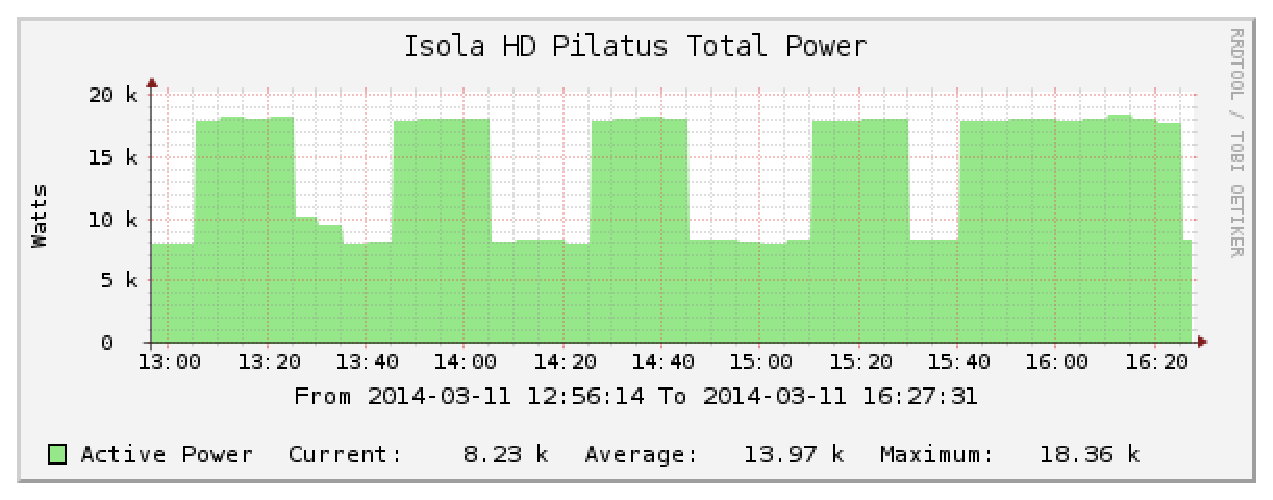
\includegraphics[width=0.48\textwidth]{Figs/NRJ_benchmark_Pilatus.eps}
  \caption{Isola HD total power dissipation of \pilat.}
  \label{fig:2}
\end{figure}

\begin{table}[htbf]
  \centering
  \caption{Averaged power dissipation (W) of the platforms.}
  \label{tab:1}
  \begin{tabular}{cccc}
    \hline\noalign{\smallskip}   \textbf{\scriptsize{Xeon   E5}}   &
    \textbf{\scriptsize{Ivy   Bridge}}   &  \textbf{\scriptsize{Xeon
        E5645}}   &   \textbf{\scriptsize{Xeon   E5645}}  \\   &   &
    \textbf{\scriptsize{(Polling)}}                                 &
    \textbf{\scriptsize{(Blocking)}}
    \\   \noalign{\smallskip}\hline\noalign{\smallskip}   18035.0  &
    12622.5 & 3713.6 & 3651.8 \\ \noalign{\smallskip}\hline
  \end{tabular}
\end{table}

In  Figure~\ref{fig:3}, we  compare both  TTS (right  Y-axis)  and ETS
(left  Y-axis)  metrics  on  both  platforms.  As  expected,  Xeon  E5
outperforms Ivy  Bridge EP, being roughly 130\,\%  faster.  The reason
for that is two-fold: \emph{i}) it has higher clock frequency than Ivy
Bridge  (2.6\,GHz  against  2.2\,GHz),   and  \emph{ii})  it  aims  at
computing speed regardless to energy consumption.  In our experiments,
Ivy Bridge EP showed  the best energy-to-solution, reducing the energy
consumption of Xeon E5 by approximately 7\,\%.

Averaged TTS and ETS results  over 10 repetitions of 24h simulation on
\tinto are shown in  Figure~\ref{fig:4}. The corresponding results for
the  averaged total  power are  also shown  in  Table~\ref{tab:1}.  As
expected, the average total power dissipation by \cosmoart while using
the blocking MPI policy is about  2\,\% less than that consumed by the
polling  policy. This is  due to  the power-friendly  (blocking) waits
performed  by the  CPU cores  while using  the blocking  MPI  mode, in
contrast to  the polling  waits that take  place when the  polling MPI
mode is set. From the point of  view of the execution time, there is a
slight reduction  for the blocking MPI  mode. One can  expect that the
costs of the interruptions used in the blocking MPI policy can lead to
an  increase  of  the   execution  time,  however,  applications  with
extensive computing,  as e.g.  \cosmoart, may show  better performance
with the blocking  modes. This effect works in  favor with our results
since the energy consumed is also reduced (2\,\%) just by changing the
behavior of the OpenMPI library  to the blocking policy, i.e, with the
\texttt{--mca    mpi\_yield\_when\_idle}   parameter   set    in   the
\texttt{mpirun} command.

\begin{figure}[htbf]
  \centering
  \includegraphics[width=0.5\textwidth]{Figs/Time_E2S_COSMO-ART-0.eps}
  \caption{Time-to-solution and  energy-to-solution comparison between
    Xeon E5 and Ivy Bridge-EP architectures for a 24h simulation.}
  \label{fig:3}
\end{figure}

\begin{figure}[htbf]
  \centering
  \includegraphics[width=0.5\textwidth]{Figs/Time_E2S_COSMO-ART-1.eps}
  \vspace{-1cm}
  \caption{Mean time-to-solution and  energy-to-solution on \tinto for
    a 24h simulation using the  polling and blocking MPI policies. The
    95\,\%  confidence  intervals of  Student's  $t$ distribution  (10
    samples) clearly  indicates an improvement for  blocking policy in
    both TTS and ETS.}
  \label{fig:4}
\end{figure}

\begin{figure*}[ht]
  \centering
  \hspace{0.8cm} \scalebox{0.62}{\input{Figs/24hour.pstex_t}}
  \caption{24  hours  simulation power  trace  using  the polling  and
    blocking MPI policies on \tinto.}
  \label{fig:5}
\end{figure*}

\begin{figure*}[ht]
  \centering
  \scriptsize
  Simulation of 1 hour during midday (11h--12h) leveraging the polling MPI policy \\
  \scalebox{0.5}{\input{Figs/11_12_blq0_figure.pstex_t}} \\
  Simulation of 1 hour during midday (11h--12h) leveraging the blocking MPI policy \\
  \scalebox{0.5}{\input{Figs/11_12_blq1_figure.pstex_t}} \\
  1 hour simulation during midnight (23h--24h) leveraging the polling MPI policy \\
  \scalebox{0.5}{\input{Figs/23_24_blq0_figure.pstex_t}} \\
  1 hour simulation during midnight (23h--24h) leveraging the blocking MPI policy \\
  \scalebox{0.5}{\input{Figs/23_24_blq1_figure.pstex_t}} \\
  \begin{tabular}{rlp{-0.2cm}rlp{-0.2cm}rlp{-0.2cm}rlp{-0.2cm}rl}
    & &  & &  & &  \\[-0.15cm]
    Computation     & \multicolumn{1}{>{\columncolor[RGB]{  0,  , 255}}p{0.4cm}}{} & & 
    Block. send     & \multicolumn{1}{>{\columncolor[RGB]{255,  0,174}}p{0.4cm}}{} & & 
    Synchronization & \multicolumn{1}{>{\columncolor[RGB]{179,  0,  0}}p{0.4cm}}{} & & 
    Wait/Wait all   & \multicolumn{1}{>{\columncolor[RGB]{235,255,  0}}p{0.4cm}}{} \\
    & &  & &  & &  \\[-0.15cm]
    Immediate recv. & \multicolumn{1}{>{\columncolor[RGB]{100,100,177}}p{0.4cm}}{} & &
    Waiting a msg.  & \multicolumn{1}{>{\columncolor[RGB]{255,  0  ,0}}p{0.4cm}}{} & & 
    Group comm.     & \multicolumn{1}{>{\columncolor[RGB]{255,144, 26}}p{0.4cm}}{} & &
    Others          & \multicolumn{1}{>{\columncolor[RGB]{192,224,  0}}p{0.4cm}}{} \\
    %I/O             & \multicolumn{1}{>{\columncolor[RGB]{172,174, 41}}p{0.4cm}}{} & &
    %
    %Idle            & \multicolumn{1}{>{\columncolor[RGB]{117,195,255}}p{0.4cm}}{} \\
  \end{tabular}
  \caption{Power-performance   traces  during   midday   and  midnight
    leveraging the polling and blocking MPI policies on \tinto.}
  \label{fig:6}
\end{figure*}

\subsection{Power-performance profiling and tracing}
\label{subsec:4.3}

A full tracing  experiment is conducted on \tinto  in order to capture
an overall power profile at a much finer resolution using the attached
PDUs in each  node. First we run \cosmoart for  a 1-day simulation and
analyze the  power consumption.  Second we correlate  performance with
power  traces  of two  1-hour  time  frames  during the  day:  mid-day
(11h--12h) and midnight (23h--24h). All the experiments were performed
using 192 cores using 12 MPI processes per node on \tinto.

In order to obtain an initial overview of the power dissipation of the
system  model,  we  obtained  power  profiles  leveraging  our  \pmlib
power-measurement    framework   over    a    1-day   simulation    of
\cosmoart. These profiles, produced with both polling and blocking MPI
policies,  are depicted in  Figure~\ref{fig:5}. The  first observation
for the polling MPI policy is that the first and last hours of the day
dissipate slightly less power than  the mid-day hours. We relate these
variations  due   to  the  different   chemical  reactions,  aerosols,
radiations  and clouds  formation processes,  computed by  ART, taking
place during  daylight hours  but not during  night. In this  case the
peak power consumption is about  3821\,W. Looking at the power profile
using the blocking  MPI policy, we observe that  the 1-hour pattern is
repeated along  the 24-hours, favoring  the reduction of  power during
night  hours in  a  more noticeable  way  than that  with the  polling
policy.  The peak  power dissipation  during  day hours  of while  the
blocking  MPI policy  is leveraged  is  about 3768\,W,  which means  a
reduction of around  50\,W with respect to the  polling mode. Also, we
notice systematic  power drops for  each simulated hour.  We associate
them  to periods  in  which  the processes  were  blocked waiting  for
incoming messages  or synchronizations, thus  yielding the CPU  to low
usage. Our final observation is the reduction of the TTS by 2\,\% with
respect to the blocking MPI policy.

To  gain  more  insights   about  the  power-performance  behavior  of
\cosmoart,  we  obtained power-per\-for\-man\-ce  traces  to allow  us
correlate  the type  of  tasks  being executed  with  the total  power
dissipation  along  the   time  (see  Figure~\ref{fig:6}).   For  this
experiment we  limit the simulation  time to 1 hour  because \emph{i})
the  pattern of  the computation  performed by  \cosmoart  is repeated
hourly and, \emph{ii}) the weight  of a 1-day simulation trace can not
be easily handled using our  machines and memory available (each trace
file was about 45\,GB). To  face the problem we shrink the simulations
to 1 hour  and test a time  frame during midday (from 11h  to 12h) and
midnight  (from 23h  to  24h), in  which  \cosmoart perform  different
internal computations.  At  the same time we leverage  the two already
stated MPI policies: polling and blocking.

All  the  traces  in   Figure~\ref{fig:6}  are  divided  in  different
computation  phases. In first  phase all  the processes  perform group
communications      and       execute      MPI-receive      primitives
(e.g. \texttt{MPI\_Recv}). The second one performs computation bursts,
combined  in  between   with  group  communications,  blocking  sends,
immediate  receives and  MPI-wait primitives  are  executed.  Finally,
group  communications interlaced  with computation  and  a significant
synchronization  phase are  performed. From  the performance  point of
view, one can notice a reduction of 2\,\% in the TTS that blocking MPI
mode leads over the polling MPI  policy. On the other hand an averaged
reduction of power dissipation of  2\,\% is attained with the blocking
MPI policy  only in  routines that actually  perform synchronizations,
group  communications  and  MPI-receive/-wait primitives.   Thus,  the
reduction of the power-energy  pair directly depends on the percentage
of time in which blocking MPI  operations are executed. For the 1 hour
simulation traces, an average of 50\,\% of the time the processes were
blocked.  Taking  into account that  the total power  reduction during
blocking phases  is about 5\,\%,  one can compute an  approximation of
the  power savings,  i.e., $50\,\%  \times  5\,\% =  2.5\%$, which  is
consistent  power  reduction  obtained  for  the  full-day  simulation
(around  2\,\%). However,  we  expect higher  power-energy savings  if
future architectures tend proportional computing~\citep{Barroso-2007}.

% \begin{figure*}[htbf]
%   \centering
%   Simulation of 1 hour during midnight (from 23h to 24h) leveraging the polling MPI policy\\
%   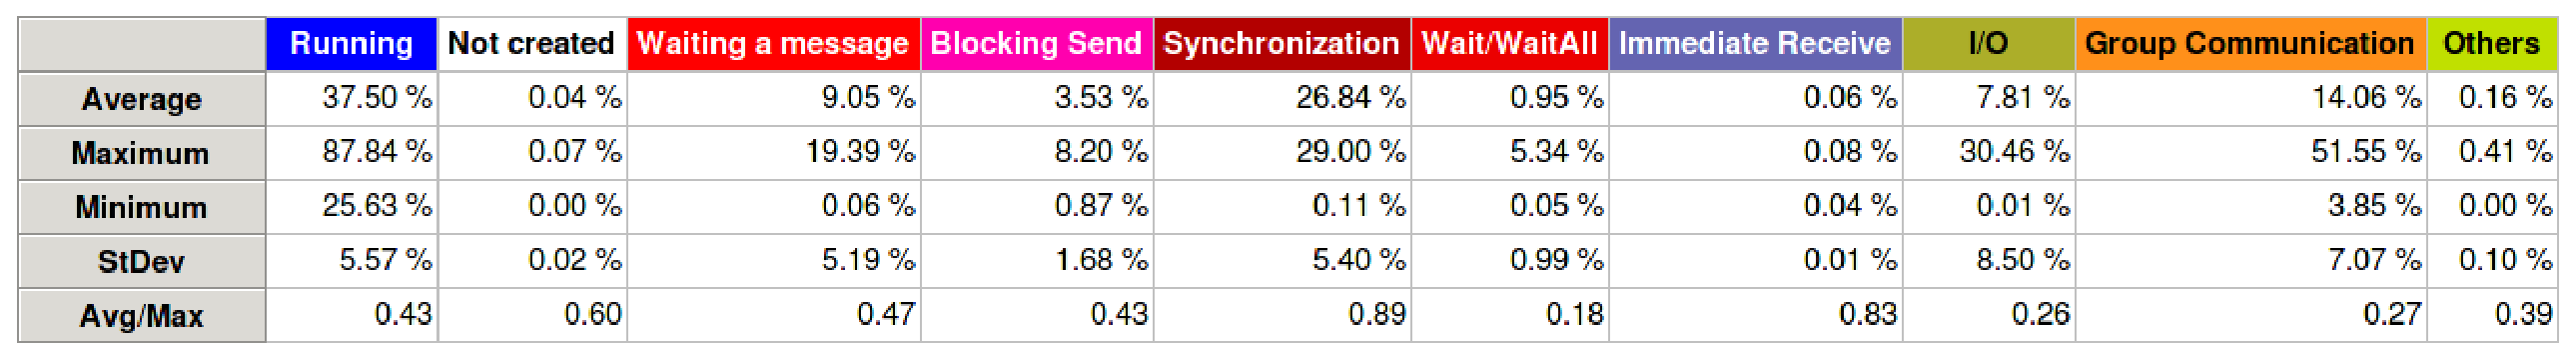
\includegraphics[width=0.78\textwidth]{Figs/23_24_blq0_stat.eps}\\
%   Percentage of time for the 1 hour during midnight (from 23h to 24h) leveraging the polling MPI policy\\
%   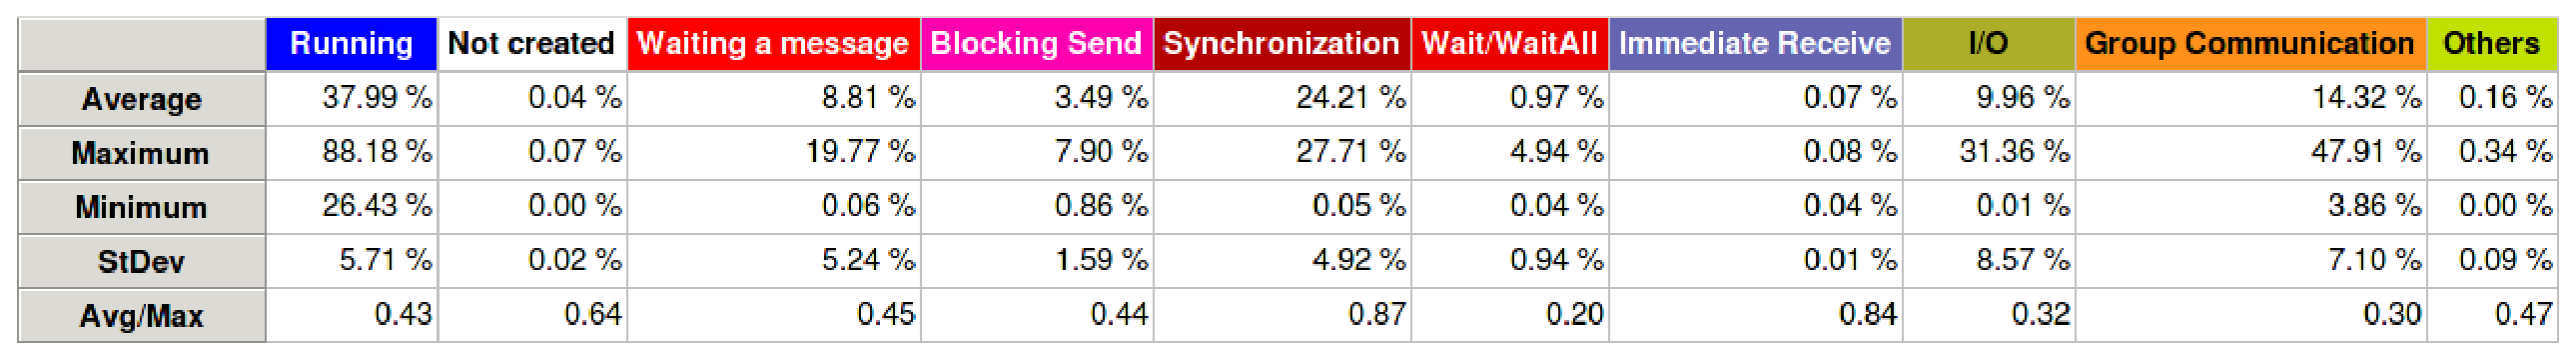
\includegraphics[width=0.78\textwidth]{Figs/23_24_blq1_stat.eps}\\
%   \caption{blabla}
%   \label{fig:7}
% \end{figure*}




\section{Conclusion}
\label{concl}
We  have   presented  a  methodology  for   comparing  performance  of
COSMO-ART,  a  regional  weather  forecast  model  augmented  for  the
interactions of  reactive gases and aerosol  particles.  The resulting
benchmarks illustrate  that the  best time-to-solution does  not imply
the best energy-to-solution: an Intel Sandybridge (2.6 GHz) system has
lower  time-to-solution but  higher energy-to-solution  than  an Intel
Ivybridge  (2.2  GHz) system,  although  the  two  metrics are  indeed
strongly  correlated. On the other hand, the usage of energy-friendly MPI waiting techniques analzyed with our power-performance framework over a series of runs of \cosmoart on \tinto and
power traces demonstrate that it is possible to reduce both
power dissipation and energy-to-solution while maintaining (or even decreasing) the time-to-solution. The  resulting profiles indicate that simple
changes, such as making use of the blocking MPI policy rather
than the polling is possible to slightly reduce both power dissipation and energy consumption (by 2\,\%).

This  reproducible  benchmark provides  a  baseline  for ongoing  work
package within  the EU-funded Exa2Green to  minimise power consumption
of COSMO-ART. Profiling  has given us insight into  the most expensive
code  components,  which are  now  being  altered  to utilise  revised
algorithms.  The  results of these  optimisations will be  reported in
future publications.


%\paragraph{Paragraph headings} Use paragraph headings as needed.

\begin{acknowledgements}
The research  leading to these  results is supported by  the Exa2Green
project  co-financed by  the European  Commission under  7th Framework
Programme Future and Emerging Technologies (FET) Proactive Initiative:
Minimising Energy  Consumption of Computing to the  Limit (MINECC). We
also gratefully acknowledge the High Performance and High Productivity
Computing Initiative  \citep{HP2C} for results that  will be leveraged
in subsequent code refactoring.
\end{acknowledgements}

\DeclareRobustCommand\IPCClongname{ - Intergovernmental Panel on Climate Change}

\bibliographystyle{plainnat}
\bibliography{\jobname}

\end{document}

